\chapter{Источники излучения}\label{radiation}
FAINA позволяет рассчитывать электромагнитное излучение от источников с заданными функциями распределения излучающих частиц и другими параметрами.

\section{Функции распределения частиц}

Важнейшими исходными данными для расчета любого типа излучения является функция распределения излучающих частиц. В коде FAINA для представления распределений используется абстрактный класс ParticleDistribution и семейство наседованных от него классов, соответствующих различным конкретным реализациям. Класс ParticleDistribution имеет следующие доступные методы, описанные в Таблице \ref{ParticleDistribution}:

	\begin{table}
	\begin{center}
		\caption{Публичные методы класса ParticleDistribution }
		\label{ParticleDistribution}
		\begin{small}
		\begin{tabularx}{\textwidth}{|X|X|}
			\hline
			\textbf{ParticleDistribution} & Абстрактный класс для любых распределений частиц\\
			\hline
			double distribution(const double\& energy, const double\& mu, const double\& phi) & возвращает функцию распределения от энергии, косинуса полярного угла и азимутального угла, нормированную на концентрацию \\
			\hline
			virtual double distributionNormalized(const double\& energy, const double\& mu, const double\& phi) & чисто виртуальный метод, возвращает функцию распределения от энергии, косинуса полярного угла и азимутального угла, нормированную на единицу \\
			\hline
			virtual double getMeanEnergy() & чисто виртуальный метод, возвращает значение средней энергии частиц в распределении\\
			\hline
			double getConcentration() & возвращает концентрацию частиц\\
			\hline
			void resetConcentration(const double\& concentration) & изменяет концентрацию на новое значение \\
			\hline
		\end{tabularx}
	    \end{small}
	\end{center}
\end{table}

Для вычисления излучения необходимо в первую очередь задать распределение излучающих частиц. Для это нужно создать объект из подходящего класса-наследника ParticleDistribution. Дерево наследования этого класс делится на две большие ветви - распределения фотонов, представленных абстрактным классом PhotonDistribution и распределения массивных частиц - MassiveParticleDistribution. Схема наследования этих классов представлена на рисунке \ref{particleDistribution0}. 

\begin{figure}
	\centering
	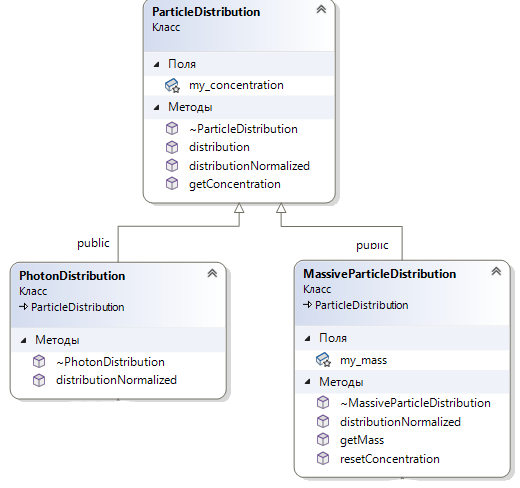
\includegraphics[width=8.5 cm]{./fig/particleDistribution0.png} 
	\caption{Схема наследования распределения фотонов и массивных частиц}
	\label{particleDistribution0}
\end{figure}

Важно отметить, что распределения фотонов не используются для представления результатов расчета излучения. Они нужны как входной параметр для расчета обратного комптоновского рассеяния. Класс PhotonDistribution не имеет дополнительных собственных методов и является лишь интерфейсом. Класс MassiveParticleDistribution тоже является абстрактным, в нем не задан конкретный вид распределения, но добавлены новые методы, описанные в Таблице \ref{MassiveParticleDistribution}	
\begin{table}
	\begin{center}
		\caption{Публичные методы класса MassiveParticleDistribution }
		\label{MassiveParticleDistribution}
		\begin{small}
			\begin{tabularx}{\textwidth}{|X|X|}
				\hline
				\textbf{MassiveParticleDistribution} & Абстрактный класс для распределений массивных излучающих частиц\\
				\hline
				virtual double minEnergy() & чисто виртуальный метод, возвращает нижнюю границу энергии частиц в распределении\\
				\hline
				virtual double maxEnergy() & чисто виртуальный метод, возвращает верхнюю границу энергии частиц в распределении. ОБРАТИТЕ ВНИМАНИЕ! если распределение не ограничено по энергии, возвращается отрицательное число.\\
				\hline
				double getMass() & возвращает массу частиц \\
				\hline
			\end{tabularx}
		\end{small}
	\end{center}
\end{table}
\subsection{Распределения фотонов}

От абстрактного класса PhotonDistribution наследуются следующие классы: абстрактный PhotonIsotropicDistribution, предназначенный для представления изотропных распределений фотонов, PhotonPlankDirectedDistribution, представляющий планковское распределение по энергии, но сконцентрированное в некотором телесном угле, такое распределение удобно для модели излучения звезды на некотором расстоянии от нее, и CompoundPhotonDistribution, представляющий из себя сумму нескольких распределений фотонов общего вида.

У изотропного распределения PhotonIsotropicDistribution добавляются методы, возвращающие значение функции распределения только в зависимости от энергии. Важно понимать, что это не функция распределения по энергии, а полная функция распределения с отброшенными угловыми аргументами. Другими словами, для получения значения функции распределения по энергии нужно домножить значение, возвращенное данным методом на $4 \pi$.
У класса PhotonIsotropicDistribution есть четыре наследника, которые являются не абстрактными классами, а непосредственно предназначены для создания распределений. Это PhotonPowerLawDistribution для представления степенных распределений, PhotonPlankDistribution, для планковских распределений, PhotonMultiPlankDistribution, для суммы планковских распределений, и PhotonMonoenergeticDistribution для моноэнергетичного изотропного распределения. Схема наследования классов фотонных распределений представлена на рисунке \ref{photonDistribution}.

\begin{figure}
	\centering
	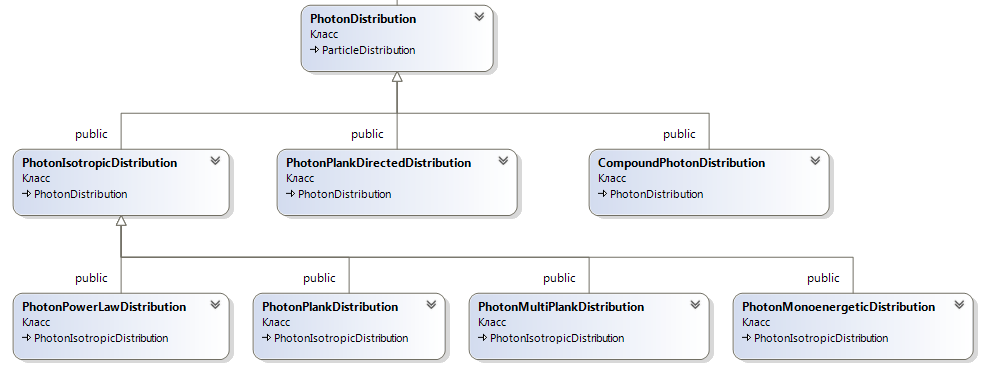
\includegraphics[width=10.5 cm]{./fig/photonDistribution2.png} 
	\caption{Схема наследования классов распределений фотонов}
	\label{photonDistribution}
\end{figure}

Методы класса PhotonDistribution и его наследников перечислены в таблице \ref{photonDistributionMethods}

\begin{small}
	\topcaption{Публичные методы классов распределений фотонов }
	\label{photonDistributionMethods}
	\begin{xtabular}{|p{0.45\textwidth}|p{0.55\textwidth}|}
				\hline
				\textbf{PhotonIsotropicDistribution} & Абстрактный класс для изотропных распределений фотонов\\
				\hline
				double distribution(const double\& energy) & возвращает функцию распределения с отброшенными угловыми аргументами, то есть нормированную на концентрацию, деленную на $4 \pi$ \\
				\hline
				virtual double distributionNormalized(const double\& energy) & чисто виртуальный метод, возвращает функцию распределения с отброшенными угловыми аргументами, нормированную на  $ 1 / 4 \pi$\\
				\hline
				void writeDistribution(const char* fileName, int Ne, const double\& Emin, const double\& Emax) & записывает распределение в файл в виде двух столбцов с точками распределенными логарифмически\\
				\hline
				\textbf{PhotonPowerLawDistribution} & Класс для степенного распределения фотонов\\
				\hline
				PhotonPowerLawDistribution(const double\& index, const double\& E0, const double\& concentration) & конструктор, создающий экземпляр с заданными показателем наклона, начальной энергией и полной концентрацией \\
				\hline
				double getIndex() & возвращает показатель наклона спектра\\
				\hline
				double getE0() & возвращает минимальную энергию степенного распределения\\
				\hline
				\textbf{PhotonPlankDistribution} & Класс для планковского распределения фотонов\\
				\hline
				PhotonPlankDistribution(const double\& temperature, const double\& amplitude) & конструктор, создающий экземпляр с заданными температурой и апмплитудой - то есть отношением концентрации к равновесному планковскому распределению с данной температурой\\
				\hline
				static PhotonPlankDistribution* getCMBRadiation() & статический метод, возвращающий экземпляр, соответствующий реликтовому излучению (температура $2.725 K$, амплитуда $1$)\\
				\hline
				double getTemperature() & возвращает температуру распределения\\
				\hline
				\textbf{PhotonMultiPlankDistribution} & Класс для распределения фотонов, состоящего из суммы планковских распределений\\
				\hline
				PhotonMultiPlankDistribution(int Nplank, const double* const temperatures, const double* const amplitudes) & конструктор, принимающий количество планковских распределений, участвующих в смеси, массив их температур и массив амплитуд\\
				\hline
				static PhotonMultiPlankDistribution* getGalacticField() & статический метод, возвращающий экземпляр, соответствующий среднегалактическому фотонному распределению, по данным статьи \cite{Mathis1983}. Данное распределение состоит из пяти планковских компонент, с температурами $2.725K, 20K, 3000K, 4000K, 7000K$ и амплитудами $1.0, 4\cdot10^{-4}, 4\cdot10^{-13}, 1.65\cdot10^{-13}, 1.0\cdot10^{-14}$ соответственно\\
				\hline
				\textbf{PhotonMonoenergeticDistribution} & Класс для моноэнергетического изотропного распределения фотонов\\
				\hline
				PhotonMonoenergeticDistribution(const double\& Energy, const double\& halfWidth, const double\& concentration) & конструктор, принимающий среднюю энергию распределения, полуширину разброса вокруг нее и концентрацию\\
								\hline
				\textbf{CompoundPhotonDistribution} & Класс для распределения фотонов, состоящего из суммы других распределений\\
				\hline
				CompoundPhotonDistribution(int N, PhotonDistribution** distributions) & конструктор, создающий экземпляр с заданным количеством распределений в смеси и массивом этих распределений \\
				\hline
				CompoundPhotonDistribution( PhotonDistribution* dist1, PhotonDistribution* dist2) & конструктор, создающий экземпляр содержащий смесь из двух распределений\\
				\hline
				CompoundPhotonDistribution( PhotonDistribution* dist1, PhotonDistribution* dist2, PhotonDistribution* dist3) & конструкторб создающий экземпляр содержащий смесь из трех распределений\\
								\hline
				\textbf{PhotonPlankDirectedDistribution} & Класс для направленного планковского распределения фотонов\\
				\hline
				PhotonPlankDirectedDistribution(const double\& temperature, const double\& amplitude, const double\& theta0, const double\& phi0, const double\& deltaTheta) & конструктор, принимающий температуру, амплитуду, углы задающие направление излучения и угол задающий полуширину раствора конуса излучения\\
				\hline
				double getTemperature() & возвращает температуру распределения\\
				\hline
	\end{xtabular}
\end{small}


Пользователь может реализовать другие виды  излучений самостоятельно, создав класс, наследующий от PhotonDistribution или PhotonIsotropicDistribution определив необходимый виртуальный метод distributionNormalized.


\subsection{Распределения массивных частиц}
Распределения массивных частиц представлены наследниками класса MassiveParticleDistribution. Так же как и в случае с фотонами важную роль играет абстрактный клас для представления изотропных распределений - MassiveParticleIsotropicDistribution. У этого класса есть методы возвращающие значение функции распределения в зависимости от энергии, и опять же, это не функция распределения, проинтегрированная по углам, а полная функция распределения с отброшенными угловыми аргументами. Для получения значения функции распределения по энергии нужно домножить значение, возвращенное данным методом на $4 \pi$. 

Абстрактный класс изотропных распределений имеет семь наследников, предназначенных для создания конкретных распределений: MassiveParticlePowerLawDistribution - для степенных распределений, MassiveParticleBrokenPowerLawDistribution - для степенных распределений с изломом, MassiveParticlePowerLawCutoffDistribution - для степенных распределений с экспоненциальным завалом, MassiveParticleMaxwellDistribution - для максвелловского распределения (обратите внимание, что в отличие от остальных распределений, максвелловское подразумевает под энергией только кинетическую энергию), MassiveParticleMaxwellJuttnerDistribution - для релятивистского распределения Максвелла-Юттнера, MassiveParticleTabulatedIsotropicDistribution - для таблично заданных распределений и MassiveParticleMonoenergeticDistribution - для моноэнергичного изотропного распределения.

Так же имеется шесть реализаций анизотропных распределений: MassiveParticleTabulatedPolarDistribution - для таблично заданных распределений с зависимостью только от энергии и полярного угла, MassiveParticleAnisotropicDistribution - для таблично заданных распределений с зависимостью от всех переменных, MassiveParticleMonoenergeticDirectedDistribution - для моноэнергичного пучка частиц, с импульсами направленными в заданный телесный угол, MassiveParticleMovingDistribution - для перевода функций распределения в движущуюся систему отсчета, CompoundMassiveParticleDistribution - для суммы распредлений общего вида, CompoundWeightedMassiveParticleDistribution - для взвешенной суммы распределений общего вида. В некоторых случаях оперировать весами распределений удобнее, чем непосредственно концентрациями. Полная схема наследования классов распределений массивных частиц представлена на рисунке \ref{massiveDistribution}. 

\begin{figure}[h]
	\centering
	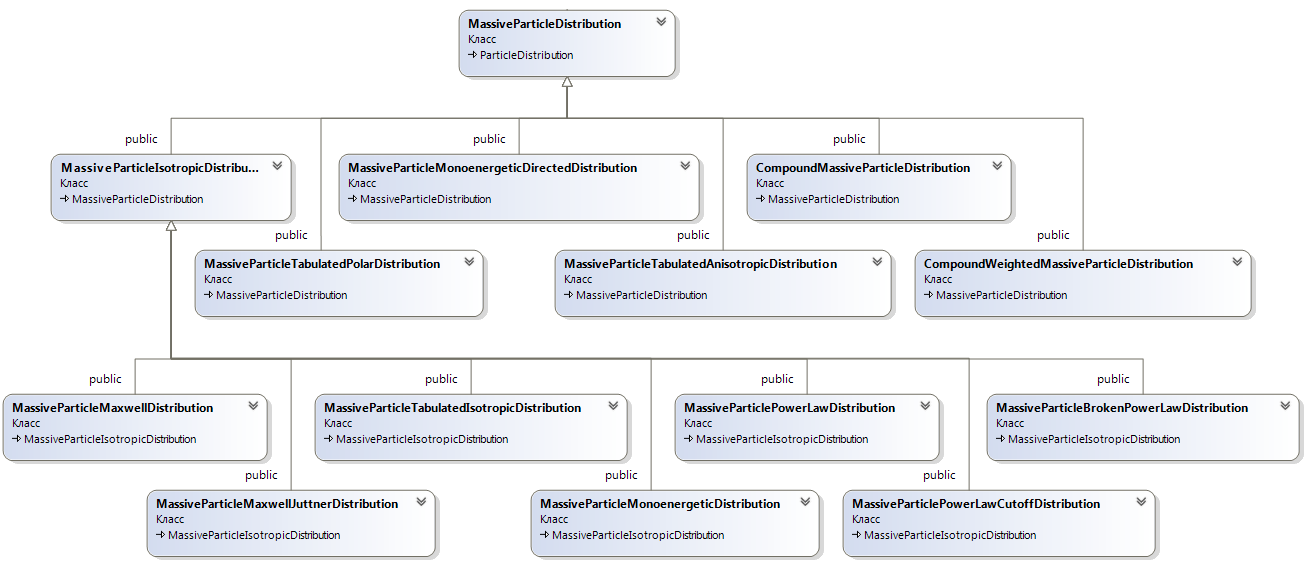
\includegraphics[width=14.5 cm]{./fig/massiveParticleDistribution2.png} 
	\caption{Схема наследования классов распределения массивных частиц}
	\label{massiveDistribution}
\end{figure}

Cписок публичных методов классов распределений массивных частиц приведен в Таблице \ref{MassiveParticleMethods}.Пользователь может сам реализовывать необходимые ему виды распределений излучающих частиц, создав наследника класса MassiveParticleDistribution или MassiveParticleIsotropicDistribution и определив необходимые виртуальные методы.

\begin{small}
		\topcaption{Публичные методы классов распределений массивных частиц }
		\label{MassiveParticleMethods}
			\begin{xtabular}{|p{0.57\textwidth}|p{0.43\textwidth}|}
				\hline
				\textbf{MassiveParticleIsotropicDistribution} & Абстрактный класс для изотропных распределений\\
				\hline
				double distribution(const double\& energy) & возвращает функцию распределения с отброшенными угловыми аргументами, то есть нормированную на концентрацию, деленную на $4 \pi$ \\
				\hline
				virtual double distributionNormalized(const double\& energy) & чисто виртуальный метод, возвращает функцию распределения с отброшенными угловыми аргументами, нормированную на  $ 1 / 4 \pi$\\
				\hline
				void writeDistribution(const char* fileName, int Ne, const double\& Emin, const double\& Emax) & записывает распределение в файл с данным именем, в диапазоне межджу данными минимальной и максимальной енергиями с заданным количеством точек, которые распределяются логарифмически\\
				\hline
				double distributionNormalizedWithLosses( const double\& energy, const double\& lossRate, const double\& time) & возвращает распределение с учетом эволюции во времени за счет синхротронных потерь до времени t определяемое уравнением $f_t(E)=f\left(\frac{E}{1-E l t}\right)\cdot\frac{1}{\left(1- E l t\right)^2}$ and loss rate $l = 4e^4 B^2 /9m^4 c^7$\\
				\hline
				\textbf{MassiveParticlePowerLawDistribution} & Класс для степенного распределения\\
				\hline
				MassiveParticlePowerLawDistribution( const double\& mass, const double\& index, const double\& E0, const double\& concentration) & конструктор, создает экземпляр степенного распределния частиц с заданными массой, степенным индексом, начальной энергией распределения и полной концентрацией\\
				\hline
				double getIndex() & возвращает степенной индекс распределения\\
				\hline
				double getE0() & возвращает начальную энергию распределения\\
				\hline
				\textbf{MassiveParticleBrokenPowerLawDistribution} & Класс для степенного распределения с изломом\\
				\hline
				MassiveParticleBrokenPowerLawDistribution( const double\& mass, const double\& index1, const double\& index2, const double\& E0, const double\& Etran, const double\& concentration) & конструктор, создает экземпляр степенного распределния с изломом частиц с заданными массой, степенными индексоми на низких и высоких энергиях, начальной энергией распределения, энергией соответствующей излому и полной концентрацией\\
				\hline
				double getIndex1() & возвращает степенной индекс распределения на низких энергиях\\
				\hline
				double getIndex2() & возвращает степенной индекс распределения на высоких энергиях\\
				\hline
				double getE0() & возвращает начальную энергию распределения\\
				\hline
				double getEtran() & возвращает энергию излома\\
				\hline
				\textbf{MassiveParticlePowerLawCutoffDistribution} & Класс для степенного распределения с экспоненциальным завалом\\
				\hline
				MassiveParticlePowerLawCutoffDistribution(const double\& mass, const double\& index, const double\& E0, const double\& beta, const double\& Ecut, const double\& concentration) & конструктор, создает экземпляр степенного распределния с экспоненциальным завалом частиц с заданными массой, степенным индексом, начальной энергией распределения, параметром завала, энергией завала и полной концентрацией. $F(E)\propto (E/E_0)^{-index}\cdot\exp(-(E/E_{cut})^\beta)$\\
				\hline
				double getIndex() & возвращает степенной индекс распределения \\
				\hline
				double getBeta() & возвращает параметр завала распределения \\
				\hline
				double getE0() & возвращает начальную энергию распределения\\
				\hline
				double getEcutoff() & возвращает энергию экспоненциального завала\\
				\hline
				\textbf{MassiveParticleMaxwellDistribution} & Класс для распределения Максвелла\\
				\hline
				MassiveParticleMaxwellDistribution( const double\& mass, const double\& temperature, const double\& concentration) & конструктор, создает экземпляр распределния Максвелла частиц с заданными массой, температурой и полной концентрацией\\
				\hline
				double getTemperature() & возвращает температуру распределения\\
				\hline
				\textbf{MassiveParticleMaxwellJuttnerDistribution} & Класс для распределения Максвелла-Юттнера\\
				\hline
				MassiveParticleMaxwellJuttnerDistribution( const double\& mass, const double\& temperature, const double\& concentration) & конструктор, создает экземпляр распределния Максвелла-Юттнера частиц с заданными массой, температурой и полной концентрацией\\
				\hline
				double getTemperature() & возвращает температуру распределения\\
				\hline
				\textbf{MassiveParticleTabulatedIsotropicDistribution} & Класс для таблично заданного изотропного распределения\\
				\hline
				MassiveParticleTabulatedIsotropicDistribution( const double\& mass, const char* fileName, const int N, const double\& concentration, DistributionInputType inputType) & конструктор, создает экземпляр табличного распределния частиц с заданными массой и полной концентрацией с помощью указанного файла, состоящего из двух колнок с данными указанной длины. Так же указывается формат входных данных.\\
				\hline
				MassiveParticleTabulatedIsotropicDistribution( const double\& mass, const char* energyFileName, const char* distributionFileName, const int N, const double\& concentration, DistributionInputType inputType) & конструктор, создает экземпляр табличного распределния частиц с заданными массой и полной концентрацией с помощью указанных двух файлов, состоящих из колнок с данными указанной длины. Так же указывается формат входных данных. \\
				\hline
				MassiveParticleTabulatedIsotropicDistribution( const double\& mass, const double* energy, const double* distribution, const int N, const double\& concentration, DistributionInputType inputType) & конструктор, создает экземпляр табличного распределния частиц с заданными массой и полной концентрацией с помощью двух переданных массивов данных указанной длины. Так же указывается формат входных данных.\\
				\hline
				int getN() & возвращает количество ячеек в таблице задающей функцию\\
				\hline
				double rescaleDistribution(const double\& k) & масштабирует распределение, вытягивая его по оси энергии по формуле $E' = mc^2 + k\cdot(E-mc^2)$, $F(E')=F(E)/k$. Данная функция может быть полезна, например, в случае когда исходная функция распределения получена в результате работы численного кода с измененной массой электронов\\
				\hline
				void addPowerLaw( const double\& Epower, const double\& index) & добавляет к функции распределения степенной с указанным индексом, начиная с указанной энергии. Функция распределения при этом остается нормированной на указанную ранее концентрацию\\
				\hline
				\textbf{MassiveParticleMonoenergeticDistribution} & Класс для моноэнергичного изотропного распределения\\
				\hline
				MassiveParticleMonoenergeticDistribution(const double\& mass, const double\& Energy, const double\& halfWidth, const double\& concentration) & конструктор, принимающий массу, среднюю энергию, полуширину разброса по энергии и концентрацию\\
				\hline 
				\textbf{MassiveParticleTabulatedPolarDistribution} & Класс для таблично заданного распределения с зависимостью от полярного угла\\
				\hline
				MassiveParticleTabulatedPolarDistribution( const double\& mass, const char* energyFileName, const char* muFileName, const char* distributionFileName, const int Ne, const int Nmu, const double\& concentration, DistributionInputType inputType) & конструктор, создает экземпляр табличного распределния частиц с заданными массой и полной концентрацией с помощью  трех указанных файлов, в двух из которых содержатся сетки по энергии и косинусу полярного угла с указанными размерами, а в третьем двумерный массив функции распределения. Так же указывается формат входных данных.\\
				\hline
				MassiveParticleTabulatedPolarDistribution( const double\& mass, const double* energy, const double* mu, const double** distribution, const int Ne, const int Nmu, const double\& concentration, DistributionInputType inputType) & конструктор, создает экземпляр табличного распределния частиц с заданными массой и полной концентрацией с помощью трех переданных массивов данных, в двух из которых содержатся сетки по энергии и косинусу полярного угла с указанными размерами, а в третьем двумерный массив функции распределения. Так же указывается формат входных данных.\\
				\hline
				int getNe() & возвращает количество ячеек по энергии в таблице задающей функцию распределения\\
				\hline
				int getNmu() & возвращает количество ячеек по полярному углу в таблице задающей функцию распределения\\
				\hline
				void double rescaleDistribution(const double\& k) & масштабирует распределение, вытягивая его по оси энергии по формуле $E' = mc^2 + k\cdot(E-mc^2)$, $F(E',\mu)=F(E,\mu)/k$. Данная функция может быть полезна, например, в случае когда исходная функция распределения получена в результате работы численного кода с измененной массой электронов\\
				\hline
				\textbf{MassiveParticleTabulatedAnisotropicDistribution} & Класс для таблично заданного анизотропного распределения общего вида\\
				\hline
				MassiveParticleTabulatedAnisotropicDistribution( const double\& mass, const char* energyFileName, const char* muFileName, const char* distributionFileName, const int Ne, const int Nmu, const int Nphi, const double\& concentration, DistributionInputType inputType) & конструктор, создает экземпляр табличного распределния частиц с заданными массой и полной концентрацией с помощью  трех указанных файлов, в двух из которых содержатся сетки по энергии и косинусу полярного угла с указанными размерами, а в третьем двумерный массив функции распределения. Сетка по азимутальному углу считается расномерной и определяется только размером. Так же указывается формат входных данных.\\
				\hline
				MassiveParticleTabulatedAnisotropicDistribution( const double\& mass, const double* energy, const double* mu, const double*** distribution, const int Ne, const int Nmu, const int Nphi, const double\& concentration, DistributionInputType inputType) & конструктор, создает экземпляр табличного распределния частиц с заданными массой и полной концентрацией с помощью трех переданных массивов данных, в двух из которых содержатся сетки по энергии и косинусу полярного угла с указанными размерами, а в третьем двумерный массив функции распределения. Сетка по азимутальному углу считается расномерной и определяется только размером. Так же указывается формат входных данных.\\
				\hline
				int getNe() & возвращает количество ячеек по энергии в таблице задающей функцию распределения\\
				\hline
				int getNmu() & возвращает количество ячеек по полярному углу в таблице задающей функцию распределения\\
				\hline
				int getNphi() & возвращает количество ячеек по азимутальному углу в таблице задающей функцию распределения\\
				\hline
				void rescaleDistribution(const double\& k) & масштабирует распределение, вытягивая его по оси энергии по формуле $E' = mc^2 + k\cdot(E-mc^2)$, $F(E',\mu, \phi)=F(E,\mu, \phi)/k$. Данная функция может быть полезна, например, в случае когда исходная функция распределения получена в результате работы численного кода с измененной массой электронов\\
				\hline
				\textbf{MassiveParticleMonoenergeticDirectedDistribution} & Класс для моноэнергичного направленного пучка частиц\\
				\hline
				MassiveParticleMonoenergeticDirectedDistribution(const double\& mass, const double\& Energy, const double\& halfWidth, const double\& concentration, const double\& theta0, const double\& phi0, const double\& deltaTheta) & конструктор, принимающий массу частиц, среднюю энергию, полуширину разброса, концентрацию, углы задающие направление пучка и угол полуширины раствора конуса\\
				\hline
				\textbf{MassiveParticleMovingDistribution} & Класс осуществляющий перевод функций распределения в движущуюся систему отсчета\\
				\hline
				MassiveParticleMovingDistribution( MassiveParticleDistribution* distribution, const double\& velocity) & конструктор, принимающий функцию распределения в собственной системе отсчета и скорость движения этой системы вдоль оси z относительно лабораторной системы\\
				\hline
				\textbf{CompoundMassiveParticleDistribution} & Класс для распределения, состоящего из суммы других распределений\\
				\hline
				CompoundMassiveParticleDistribution( int N, MassiveParticleDistribution** distributions) & конструктор, создает экземпляр класса содержащий смесь заданного количества указанных распределений\\
				\hline
				CompoundMassiveParticleDistribution( MassiveParticleDistribution* dist1, MassiveParticleDistribution* dist2) & конструктор, создает экземпляр класса, содержащий смесь двух распределений \\
				\hline
				CompoundMassiveParticleDistribution( MassiveParticleDistribution* dist1, MassiveParticleDistribution* dist2, MassiveParticleDistribution* dist3) & конструктор, создает экземпляр класса, содержащий смесь трех распределений\\
				\hline
				\textbf{CompoundWeightedMassiveParticleDistribution} & Класс для распределения, состоящего из взвешенной суммы других распределений \\
				\hline
				CompoundWeightedMassiveParticleDistribution( int N, const double* weights, MassiveParticleDistribution** distributions) & конструктор, создает экземпляр класса содержащий смесь заданного количества указанных распределений с заданными весами \\
				\hline
				CompoundWeightedMassiveParticleDistribution( MassiveParticleDistribution* dist1, const double\& w1, MassiveParticleDistribution* dist2, const double\& w2) & конструктор, создает экземпляр класса, содержащий смесь двух распределений с указанными весами \\
				\hline
				CompoundWeightedMassiveParticleDistribution( MassiveParticleDistribution* dist1, const double\& w1, MassiveParticleDistribution* dist2, const double\& w2, MassiveParticleDistribution* dist3, const double\& w3) & конструктор, создает экземпляр класса, содержащий смесь трех распределений с указанными весами \\
				\hline
	\end{xtabular}
\end{small}

\subsection{Считывание распределений из файла}
Классы таблично-заданных распределений, такие как например MassiveParticleTabulatedIsotropicDistribution, имеют конструктор принимающие на вход имена файлов, из которых будет считана функция распределения. Это должны быть текстовые файлы, содержащие таблицы с данными, причем формат единиц, в которых измеряется функция распределения может быть разным. Для задания формата входных файлов используется перечислимы тип DistributionInputType, имеющий пять значений:

\begin{itemize}
	\item ENERGY\_FE - во входных файлах заданы энергия и функция распределения по энергии
	\item ENERGY\_KIN\_FE - заданы кинетическая энергия и функция распределения по энергии
	\item GAMMA\_FGAMMA - задан лоренц-фактор и функция распределения по нему
	\item GAMMA\_KIN\_FGAMMA - задан лоренц-фактор, уменьшенный на единицу, и функция распределения по нему
	\item MOMENTUM\_FP - задан импульс и функция распределения по импульсу
\end{itemize}

Вне зависимости от формата входного файла, функция распределения будет преобразована к единицам энергия - распределение по энергии. С помощью этих параметров можно считывать табличные распределения из файлов, например так:

\begin{lstlisting}[language=c++]
	double electronConcentration = 1.0;
	int N = 100;
	MassiveParticleIsotropicDistribution* distribution = new
	MassiveParticleTabulatedIsotropicDistribution(massElectron,
	"energy.dat", "distribution.dat", N, electronConcentration,
	DistributionInputType::ENERGY_FE);
\end{lstlisting}

Для облегчения создания распределений из файла в сложных случаях реализован класс MassiveParticleDistributionFactory. У него есть несколько методов, позволяющих считывать целые серии распределений из набора пронумерованных файлов. Что может быть полезно, если функция распределения зависит от некоторого параметра, как в примере вычисления синхротронного излучения описанном в следующей главе \ref{}. Считать серию из десяти распределений электронов, содержащихся в файлах с именами  "Fe0.dat"\ , "Fe1.dat"\  и так далее, состоящих из двух колонок - лоренц-фактор и функция распределения, и добавить к этим распределениям степенной хвост с показателем 3, начиная с энергий в 100 энергий покоя можно вызовом одной функции: 

\begin{lstlisting}[language=c++]
	double electronConcentration = 1.0;
	int Nenergy = 100;
	int Ndistribution = 100;
	double powerLawEnergy = 100*me_c2;
	double index = 3.0;
	MassiveParticleIsotropicDistribution** distributions = 
	MassiveParticleDistributionFactory::
	readTabulatedIsotropicDistributionsAddPowerLawTail(
	massElectron, "./input/Fe", ".dat", Ndistribution, 
	DistributionInputType::GAMMA_FGAMMA, electronConcentration, Nenergy,
	powerLawEnergy, index);
\end{lstlisting}

Так же у пользователя есть возможность использовать конструкторы табличных распределений, принимающие не имена файлов, а непосредственно массивы со значениями функции распределения, которые пользователь может создать любым удобным ему способом.

\section{Источники излучения}

В коде FAINA есть возможность расчета излучения, используя на прямую функции распределения излучающих частиц, с указанием необходимых дополнительных параметров, таких как объем источника, расстояние до него, магнитное поле и других. Но более универсальным и рекомендованным способ является расчет с помощью создания модели источника излучения. При таком подходе возможно учесть геометрическое строение источника, его неоднородности и другие особенности.

Реализованы два базовых класса источников - независящие от времени, представленные абстрактным классом RadiationSource, и изменяющиеся со временем, представленные абстрактным классом RadiationTimeDependentSource. Эти два класса не связаны между собой через наследование, но объект первого класса содержится внутри объектов второго как приватное поле класса. Схема классов источников излучения представлена на рисунке \ref{radiationSource}.

\begin{figure}[h]
	\centering
	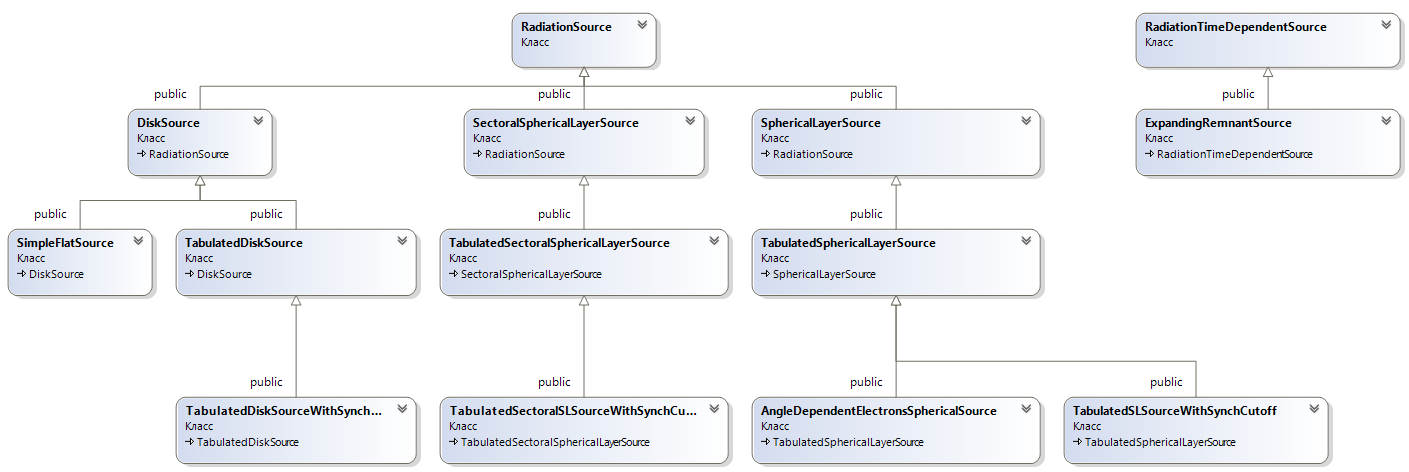
\includegraphics[width=14.5 cm]{./fig/radiationSource2.png} 
	\caption{Схема наследования классов источников излучения}
	\label{radiationSource}
\end{figure}

\subsection{Источники излучения, не зависящие от времени}\label{sourcesSection}
Источники излучения без временной зависимости реализованы с помощью абстрактного класса RadiationSource. Геометрически каждый источник задан в виде пространственной области в цилиндрических координатах, с осью z направленной вдоль луча зрения к наблюдателю, и характеризуется максимальным радиусом и минимальным и максимальным значением координаты z. Такая система координат выбрана для удобства учета процессов поглощения при прохождении излучения внутри самого источника вдоль луча зрения. Отличие реальной формы источника от цилиндрической реализовано с помощью долей заполнения веществом источника ячеек пространственной сетки. Модель источника, имеющего форму шарового слоя, в цилиндрическо пространственной сетке изображена на рисунке \ref{sphericalLayer}. Цветом обозначена доля объема ячейки, заполненная веществом источника.

\begin{figure}
	\centering
	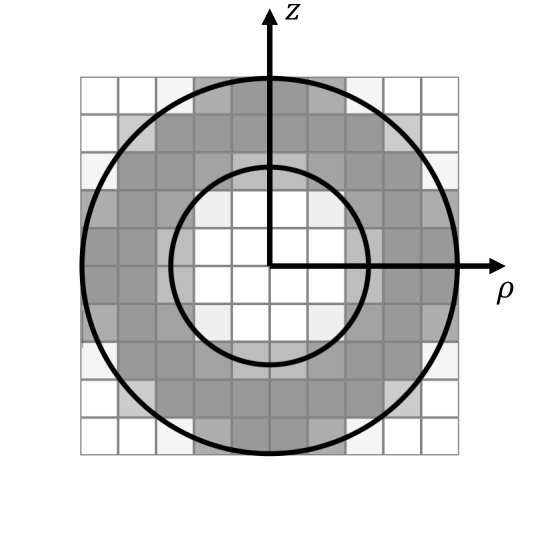
\includegraphics[width=10.5 cm]{./fig/sphericalSource.png} 
	\caption{Модель источника в форме шарового слоя, помещенного в цилиндрическую пространственную координатную сетку. Цвет характеризует долю объема ячейки, заполненную веществом источника.}
	\label{sphericalLayer}
\end{figure}

Так же источники излучения имеют следующие важные характеристки, которые могут меняться в различных пространственных ячейках источника: концентрация излучающих частиц, их функция распределения, магнитное поле и угол его наклона к лучу зрения. Большинство методов расчета излучения (все кроме обратного комптоновского рассеяния) реализованы только для изотропных распределений излучающих частиц, поэтому источники содержат только изотропные распределения. Так же у источника должно быть задано расстояние до наблюдателя.

Класс RadiationSource имеет три абстрактных класса-наследника: DiskSource - для источников в форме диска, перпендикулярного лучу зрения, и SphericalLayerSource - для источников в форме шарового слоя и SectoralSphericalLayerSource - источник, который нужен тогда, когда рассматривается только сектор шарового слоя, "долька апельсина". 

Источники в форме диска имеют три реализации: SimpleFlatSource - однородный диск, состоящий из одной пространственной ячейки с заданными параметрами, и TabulatedDiskSource - источник, в котором все характеристики таблично заданы на пространственной сетке и отнаследованный от него TabulatedDiskSourceWithSynchCutoff, который нужен для учета синхротронных потерь функции распределения. В можели данного источника считается, что распределение частиц генерирутся на границе источника (верхней грани, соответствующей ударной волне), а в дальнейшем конвекционно переносятся вглубь него, испытывая при этом синхротронные потери. Изменение функции распределения в зависимости от расстояния до границы в случае однородного поля определеяется формулой:

\begin{equation}
	f_l(E)=f\left(\frac{E}{1-4e^4 B^2 E~l/9m^4 c^7 v}\right)\cdot\frac{1}{\left(1-4e^4 B^2 E~l/9m^4 c^7 v\right)^2}
\end{equation}
где $f(E)$ исходная функция распределения, $E$ - энергия частицы, $B$ - магнитное поле, $l$ - расстояние до границы, $v$ - скорость конвекционного движения, $e$ - заряд частицы, $m$ - масса частицц, $c$ - скорость света.

Источники в форме шарового слоя имеют следующие реализации: TabulatedSphericalSource - источник, в котором все характеристики таблично заданы на пространственной сетке, и отнаследованные от него  TabulatedSLSourceWithSynchCutoff и AngleDependentElectronsSphericalSource. Первый из них нужен для учета синхротронных потерь, аналогично тому как это сделано в TabulatedDiskSourceWithSynchCutoff, а второй - для реализации важного случая, когда функция распределения излучающих частиц зависит от угла наклона магнитного поля по отношению к направлению распространения ударной волны \cite{SironiSpitkovsky2009pair, GuoSironi2014_1,Crumley2019, Romansky2018, еще}. В AngleDependentElectronsSphericalSource такие параметры, как концентрация, магнитное поле и его угол наклона к лучу зрения заданы таблично на пространственной сетке, а функция распределения излучающих частиц - в виде таблицы по углам наклона магнитного поля к направлению распространения ударной волны, которая в данном случае считается сферически симметричной. Функция распределения в каждой ячейке выбирается в зависимости от вычисленного угла наклона магнитного поля к ударной волне.

Источники в форме шарового слоя имеют следующие реализации: TabulatedSectoralSphericalLayerSource - источник, в котором все характеристики таблично заданы на пространственной сетке, и отнаследованный от него TabulatedSectoralSLSourceWithSynchCutoff, учитывающий потери энергии частиц аналогично тому, как это реализовано в классе TabulatedDiskSourceWithSynchCutoff.

Публичные методы классов источников излучения без зависимости от времени перечислены в Таблице \ref{sourceMethods1}.

\begin{small}
	\topcaption{Публичные методы классов источников излучения без зависимости от времени }
	\label{sourceMethods1}
	\begin{xtabular}{|p{0.5\textwidth}|p{0.5\textwidth}|}
		\hline
		\textbf{RadiationSource} & абстрактный класс для источников излучения общего вида\\
		\hline
		virtual double getMaxRho() & чисто виртуальный метод, возвращает границу источника по радиальной оси в цилиндрических координатах\\
		\hline
		virtual double getMinZ() & чисто виртуальный метод, возвращает минимальную границу источника по оси z\\
		\hline
		virtual double getMaxZ() & чисто виртуальный метод, возвращает максимальную границу источника по оси z\\
		\hline
		virtual double getMaxB() & чисто виртуальный метод, возвращает максимальное магнитное поле\\
		\hline
		virtual double getAverageSigma() & чисто виртуальный метод, возвращает среднюю магнетизацию $\sigma=\frac{B^2}{4\pi n m_p c^2}$\\
		\hline
		virtual double getAverageConcentration() &чисто виртуальный метод, возвращает среднюю конценрацию\\
		\hline
		virtual double getRho(int irho) & чисто виртуальный метод, возвращает радиальную координату данной ячейки\\
		\hline
		virtual double getZ(int iz)& чисто виртуальный метод, возвращает z координату данной ячейки\\
		\hline
		virtual double getPhi(int iphi)& чисто виртуальный метод, возвращает азимутальную координату данной ячейки\\
		\hline
		virtual int getRhoIndex(const double\& rho)& чисто виртуальный метод, возвращает радиальный индекс ячейки по координате\\
		\hline
		virtual bool isSource(int irho, int iphi)& чисто виртуальный метод, возвращает логическое значение - учитывать ли ячейки с данными радиальными и азимутальными координатами при расчете излучения всего источника\\
		\hline
		int getNrho() & возвращает количество пространственных ячеек по радиальной оси цилиндрических координат\\
		\hline
		int getNz() & возвращает количество пространственных ячеек по оси z цилиндрических координат\\
		\hline
		int getNphi() & возвращает количество пространственных ячеек по по азимутальному углу цилиндрических координат\\
		\hline
		double getDistance() & возвращает расстояние до источника\\
		\hline
		getArea(int irho) & возвращает поперечное сечение данной пространственной ячейки\\
		\hline
		getVolume(int irho, int iz, int iphi) & возвращает объем ячейки, занятый веществом источника. Этот метод согласован с методами getArea и getLength и возвращает их произведение\\
		\hline
		virtual getB(int irho, int iz, int iphi) & чисто виртуальный метод, возвращает значение магнитного поля в ячейке\\
		\hline
		virtual getConcentration(int irho, int iz, int iphi) & чисто виртуальный метод, возвращает значение концентрации в ячейке \\
		\hline
		virtual getSinTheta(int irho, int iz, int iphi) & чисто виртуальный метод, возвращает синус угла наклона магнитного поля к лучу зрения\\
		\hline
		virtual void getVelocity(int irho, int iz, int iphi, double\& velocity, double\& theta, double\& phi) &\\
		чисто виртуальный метод, возвращает скорость данной ячейки источника\\
		\hline
		virtual getTotalVolume() & чисто виртуальный метод, возвращает полный объем источника\\
		\hline
		virtual getLength(int irho, int iz, int iphi) & чисто виртуальный метод, возвращает среднюю толщину ячейки, заполненную веществом источника\\
		\hline
		virtual resetParameters(const double* parameters, const double* normalizationUnits) & чисто виртуальный метод, меняющий параметры источника. Список параметров, их количество, их влияние на источник определяются пользователем в конкретных реализациях класса. Принимет массив параметров и массив единиц в которых они измерены. Данный метод используется в процедурах оптимизации, либо при учете изменения источника со временем\\
		\hline
		virtual getParticleDistribution(int irho, int iz, int iphi) & чисто виртуальный метод, возвращает распределение излучающих частиц в ячейке\\
		\hline
		\textbf{DiskSource} & Абстрактный класс для источников в форме диска\\
		\hline
		\textbf{SimpleFlatSource} & Класс для источников в форме однородного диска\\
		\hline
		SimpleFlatSource( MassiveParticleDistribution* electronDistribution, const double\& B, const double\& sinTheta, const double\& rho, const double\& z, const double\& distance, const double\& velocity = 0) & конструктор, возвращает экземпляр с заданными распределением частиц, магнитным полем, синусом угла его наклона, радиусом диска, толщиной диска, расстоянием до источника и скоростью движения вещества\\
		\hline
		\textbf{TabulatedDiskSource} & Класс для источников в форме диска с таблично заданными значениями параметров\\
		\hline
		TabulatedDiskSource( int Nrho, int Nz, int Nphi, MassiveParticleDistribution* electronDistribution, double*** B, double*** sinTheta, double*** concentration, const double\& rho, const double\& z, const double\& distance, const double\& velocity = 0) & конструктор, возвращает экземпляр с заданными с помощью массивов распределением частиц, магнитным полем, синусом угла его наклона, а так же заданными радиусом диска, толщиной диска, расстоянием до источника и скоростью движения вещества\\
		\hline
		TabulatedDiskSource( int Nrho, int Nz, int Nphi, MassiveParticleDistribution* electronDistribution, const double\& B, const double\& sinTheta, const double\& concentration , const double\& rho, const double\& z, const double\& distance, const double\& velocity = 0) & конструктор, возвращает экземпляр с заданными однородными распределением частиц, магнитным полем, синусом угла его наклона, а так же заданными радиусом диска, толщиной диска, расстоянием до источника и скоростью движения вещества\\
		\hline
		\textbf{TabulatedDiskSourceWithSynchCutoff} & Класс для источников в форме диска с таблично заданными значениями параметров и учетом синхротронных потерь энергии частиц\\
		\hline
		TabulatedDiskSourceWithSynchCutoff(int Nrho, int Nz, int Nphi, MassiveParticleDistribution* electronDistribution, double*** B, double*** theta, double*** concentration, const double\& rho, const double\& z, const double\& distance, const double\& downstreamVelocity, const double\& velocity = 0) &
		конструктор, возвращает экземпляр с заданными с помощью массивов распределением частиц, магнитным полем, синусом угла его наклона, а так же заданными радиусом диска, толщиной диска, расстоянием до источника, скоростью конвекции частиц и скоростью движения вещества\\
		\hline
		TabulatedDiskSourceWithSynchCutoff(int Nrho, int Nz, int Nphi, MassiveParticleDistribution* electronDistribution, const double\& B, const double\& concentration, const double\& theta, const double\& rho, const double\& z, const double\& distance, const double\& downstreamVelocity, const double\& velocity = 0) & конструктор, возвращает экземпляр с заданными однородными распределением частиц, магнитным полем, синусом угла его наклона, а так же заданными радиусом диска, толщиной диска, расстоянием до источника, скоростью конвекции частиц и скоростью движения вещества\\
		\hline
		\textbf{SphericalLayerSource} & Абстрактный класс для источников в форме шарового слоя\\
		\hline
		double getInnerRho() & возвращает внутренний радиус шарового слоя\\
		\hline
		\textbf{TabulatedSphericalLayerSource} & Класс для источников в форме шарового слоя с таблично заданными значениями параметров\\
		\hline
		TabulatedSphericalLayerSource(int Nrho, int Nz, int Nphi, MassiveParticleDistribution* electronDistribution, double*** B, double*** sinTheta, double*** concentration, const double\& rho, const double\& rhoin, const double\& distance, const double\& velocity = 0) & конструктор, возвращает экземпляр с заданными с помощью массивов распределением частиц, магнитным полем, синусом угла его наклона к лучу зрения, а так же заданными внешним и внутренним радиусом шарового слоя, расстоянием до источника и скоростью движения вещества\\
		\hline
		TabulatedSphericalLayerSource(int Nrho, int Nz, int Nphi, MassiveParticleDistribution* electronDistribution, const double\& B, const double\& concentration, const double\& sinTheta, const double\& rho, const double\& rhoin, const double\& distance, const double\& velocity = 0) &  конструктор, возвращает экземпляр с заданными однородными распределением частиц, магнитным полем, синусом угла его наклона, а так же заданными внутренним и внешним радиусом шарового слоя, расстоянием до источника и скоростью движения вещества\\
		\hline
		\textbf{AngleDependentElectronsSphericalSource} & Класс для источников в форме шарового слоя с таблично заданными значениями концентрации и магнитного поля и функцией распределения излучающих частиц, зависящей от угла наклона магнитного поля к направлению распространения ударной волны\\
		\hline
		AngleDependentElectronsSphericalSource( int Nrho, int Nz, int Nphi, int Ntheta, MassiveParticleDistribution** electronDistributions, double*** B, double*** sinTheta, double*** phi, double*** concentration, const double\& rho, const double\& rhoin, const double\& distance, const double\& velocity = 0) & конструктор, возвращает экземпляр с заданными с помощью массивов магнитным полем, синусом угла его наклона к лучу зрения, а так же заданными внешним и внутренним радиусом шарового слоя, расстоянием до источника и скоростью движения вещества. Распределение частиц задается в виде массива табличных значений в зависимости от угла наклона магнитного поля к направлению распространения ударной волны\\
		\hline
		AngleDependentElectronsSphericalSource(int Nrho, int Nz, int Nphi, int Ntheta, MassiveParticleDistribution** electronDistributions, const double\& B, const double\& sinTheta, const double\& phi, const double\& concentration, const double\& rho, const double\& rhoin, const double\& distance, const double\& velocity = 0) & конструктор, возвращает экземпляр с заданными однородными  магнитным полем, синусом угла его наклона, а так же заданными внутренним и внешним радиусом шарового слоя, расстоянием до источника и скоростью движения вещества. Распределение частиц задается в виде массива табличных значений в зависимости от угла наклона магнитного поля к направлению распространения ударной волны\\
		\hline
		\textbf{TabulatedSLSourceWithSynchCutoff} & Класс для источников в форме шарового слоя с таблично заданными значениями параметров и учетом синхротронных потерь энергии частиц\\
		\hline
		TabulatedSLSourceWithSynchCutoff(int Nrho, int Nz, int Nphi, MassiveParticleDistribution* electronDistribution, double*** B, double*** theta, double*** concentration, const double\& rho, const double\& rhoin, const double\& distance, const double\& downstreamVelocity, const double\& velocity = 0) & конструктор, возвращает экземпляр с заданными с помощью массивов распределением частиц, магнитным полем, синусом угла его наклона к лучу зрения, а так же заданными внешним и внутренним радиусом шарового слоя, расстоянием до источника, скоростью конвекции частиц и скоростью движения вещества\\
		\hline
		TabulatedSLSourceWithSynchCutoff(int Nrho, int Nz, int Nphi, MassiveParticleDistribution* electronDistribution, const double\& B, const double\& concentration, const double\& theta, const double\& rho, const double\& rhoin, const double\& distance, const double\& downstreamVelocity, const double\& velocity = 0) & конструктор, возвращает экземпляр с заданными однородными распределением частиц, магнитным полем, синусом угла его наклона, а так же заданными внутренним и внешним радиусом шарового слоя, расстоянием до источника, скоростью конвекции частиц и скоростью движения вещества\\
		\hline
		\textbf{SectoralSphericalLayerSource} & абстрактный класс для источников в форме сектора шарового слоя (дольки апельсина)\\
		\hline
		double getRhoin() & возвращает внутренний радиус шарового слоя\\
		\hline
		\textbf{TabulatedSectoralSphericalLayerSource} & Класс для источников в форме сектора шарового слоя с таблично заданными значениями параметров\\
		\hline
		TabulatedSectoralSphericalLayerSource(int Nrho, int Nz, int Nphi, MassiveParticleDistribution* electronDistribution, double*** B, double*** theta, double*** concentration, const double\& rho, const double\& rhoin, const double\& minrho, const double\& phi, const double\& distance, const double\& velocity = 0) & конструктор, возвращает экземпляр с заданными с помощью массивов распределением частиц, магнитным полем, синусом угла его наклона к лучу зрения, а так же заданными внешним и внутренним радиусом шарового слоя, углом раствора сектора, расстоянием до источника и скоростью движения вещества\\
		TabulatedSectoralSphericalLayerSource(int Nrho, int Nz, int Nphi, MassiveParticleDistribution* electronDistribution, const double\& B, const double\& concentration, const double\& theta, const double\& rho, const double\& rhoin, const double\& minrho, const double\& phi, const double\& distance, const double\& velocity = 0) & конструктор, возвращает экземпляр с заданными однородными распределением частиц, магнитным полем, синусом угла его наклона, а так же заданными внутренним и внешним радиусом шарового слоя, углом раствора сектора, расстоянием до источника и скоростью движения вещества\\
		\hline
		\textbf{TabulatedSectoralSLSourceWithSynchCutoff} & Класс для источников в форме сектора шарового слоя с таблично заданными значениями параметров и учетом синхротронных потерь энергии частиц\\
		\hline
		TabulatedSectoralSLSourceWithSynchCutoff(int Nrho, int Nz, int Nphi, MassiveParticleDistribution* electronDistribution, double*** B, double*** theta, double*** concentration, const double\& rho, const double\& rhoin, const double\& minrho, const double\& phi, const double\& distance, const double\& downstreamVelocity, const double\& velocity = 0) & конструктор, возвращает экземпляр с заданными с помощью массивов распределением частиц, магнитным полем, синусом угла его наклона к лучу зрения, а так же заданными внешним и внутренним радиусом шарового слоя, углом раствора сектора, расстоянием до источника, скоростью конвекции частиц и скоростью движения вещества\\
		\hline
		TabulatedSectoralSLSourceWithSynchCutoff(int Nrho, int Nz, int Nphi, MassiveParticleDistribution* electronDistribution, const double\& B, const double\& concentration, const double\& theta, const double\& rho, const double\& rhoin, const double\& minrho, const double\& phi, const double\& distance, const double\& downstreamVelocity, const double\& velocity = 0) & конструктор, возвращает экземпляр с заданными однородными распределением частиц, магнитным полем, синусом угла его наклона, а так же заданными внутренним и внешним радиусом шарового слоя, углом раствора сектора, расстоянием до источника, скоростью конвекции частиц и скоростью движения вещества\\
		\hline
	\end{xtabular}
\end{small}

\subsection{Источники излучения, меняющиеся со временем}\label{timeDependentSource}
Источники излучения, учитывающие зависимость от времени, представлены абастрактным классом классом RadiationTimeDependentSource. Этот класс не является наследником класса RadiationSource, но содержит экземпляр такого класса внутри себя, чтобы использовать его для расчета излучения в конкретный момент времени. Для этого пользователь должен самостоятельно создать имплементацию виртуальной функции getRadiationSource, в которой будут вычислены параметры источника в зависимости от времени.  В текущей версии кода реализован только один наследник RadiationTimeDependentSource - ExpandingRemnantSource, представляющий собой модель расширяющегося остатка сверхновой. В данной модели предполагается, что размер источника увеличивается во времени с постоянной скоростью, магнитное поле падает обратно пропорционально размеру источника, концентрация обратно пропорционально квадрату размера а толщина шарового слоя остается постоянной. Пользователь может создавать свои классы источников с другими зависимостями параметров от времени. Публичные методы классов RadiationTimeDependentSource и ExpandingRemnantSource перечислены  в Таблице \ref{sourceTimeDependentMethods1}.

\begin{small}
	\topcaption{Публичные методы классов источников излучения учитывающих зависимость от времени }
	\label{sourceTimeDependentMethods1}
	\begin{xtabular}{|p{0.5\textwidth}|p{0.5\textwidth}|}
		\hline
		\textbf{RadiationTimeDependentSource} & Абстрактный класс для учета изменений источников излучения со временем\\
		\hline
		virtual resetParameters(const double* parameters, const double* normalizationUnits) & чисто виртуальный метод, меняющий параметры источника. Список параметров, их количество, их влияние на источник определяются пользователем в конкретных реализациях класса. Принимает массив параметров и массив единиц в которых они измерены. Данный метод применяется в процедурах оптимизации\\
		\hline
		virtual getRadiationSource(double\& time, const double* normalizationUnits) & возвращает источник излучения с параметрами соответствующими заданному моменту времени. Так же принимает на вход массив единиц, в которых измеряются параметры этого источника.\\
		\hline
		\textbf{ExpandingRemnantSource} & класс, представляющий модель расширяющегося с постоянной скоростью остатка сверхновой, имеющего форму шарового слоя постоянной толщины с однородными концентрацией и магнитным полем \\
		\hline
		ExpandingRemnantSource(const double\& R0, const double\& B0, const double\& concentration0, const double\& v, const double\& widthFraction, RadiationSource* source, const double\& t0) & конструктор, создает экземпляр класса расширяющейся сферической оболочки с заданными в момент t0 радиусом, магнитным полем, концентрацией, скоростью расширения, отношением толщины оболочки к радиусу и моделью источника. Для коректного учета изменения источника во времени важно, чтобы конретная реализация метода source->resetParameters соответствовала той,что используется в методе getRadiationSource. В данном случае подходят все перечисленные выше реализации источников не зависящих от времени\\
		\hline
	\end{xtabular}
\end{small}